\documentclass{standalone}
\usepackage{tikz}
\usetikzlibrary{patterns, positioning}
\usepackage[sfdefault]{ClearSans} %% option 'sfdefault' activates Clear Sans as the default text font
\usepackage[T1]{fontenc}

\begin{document}
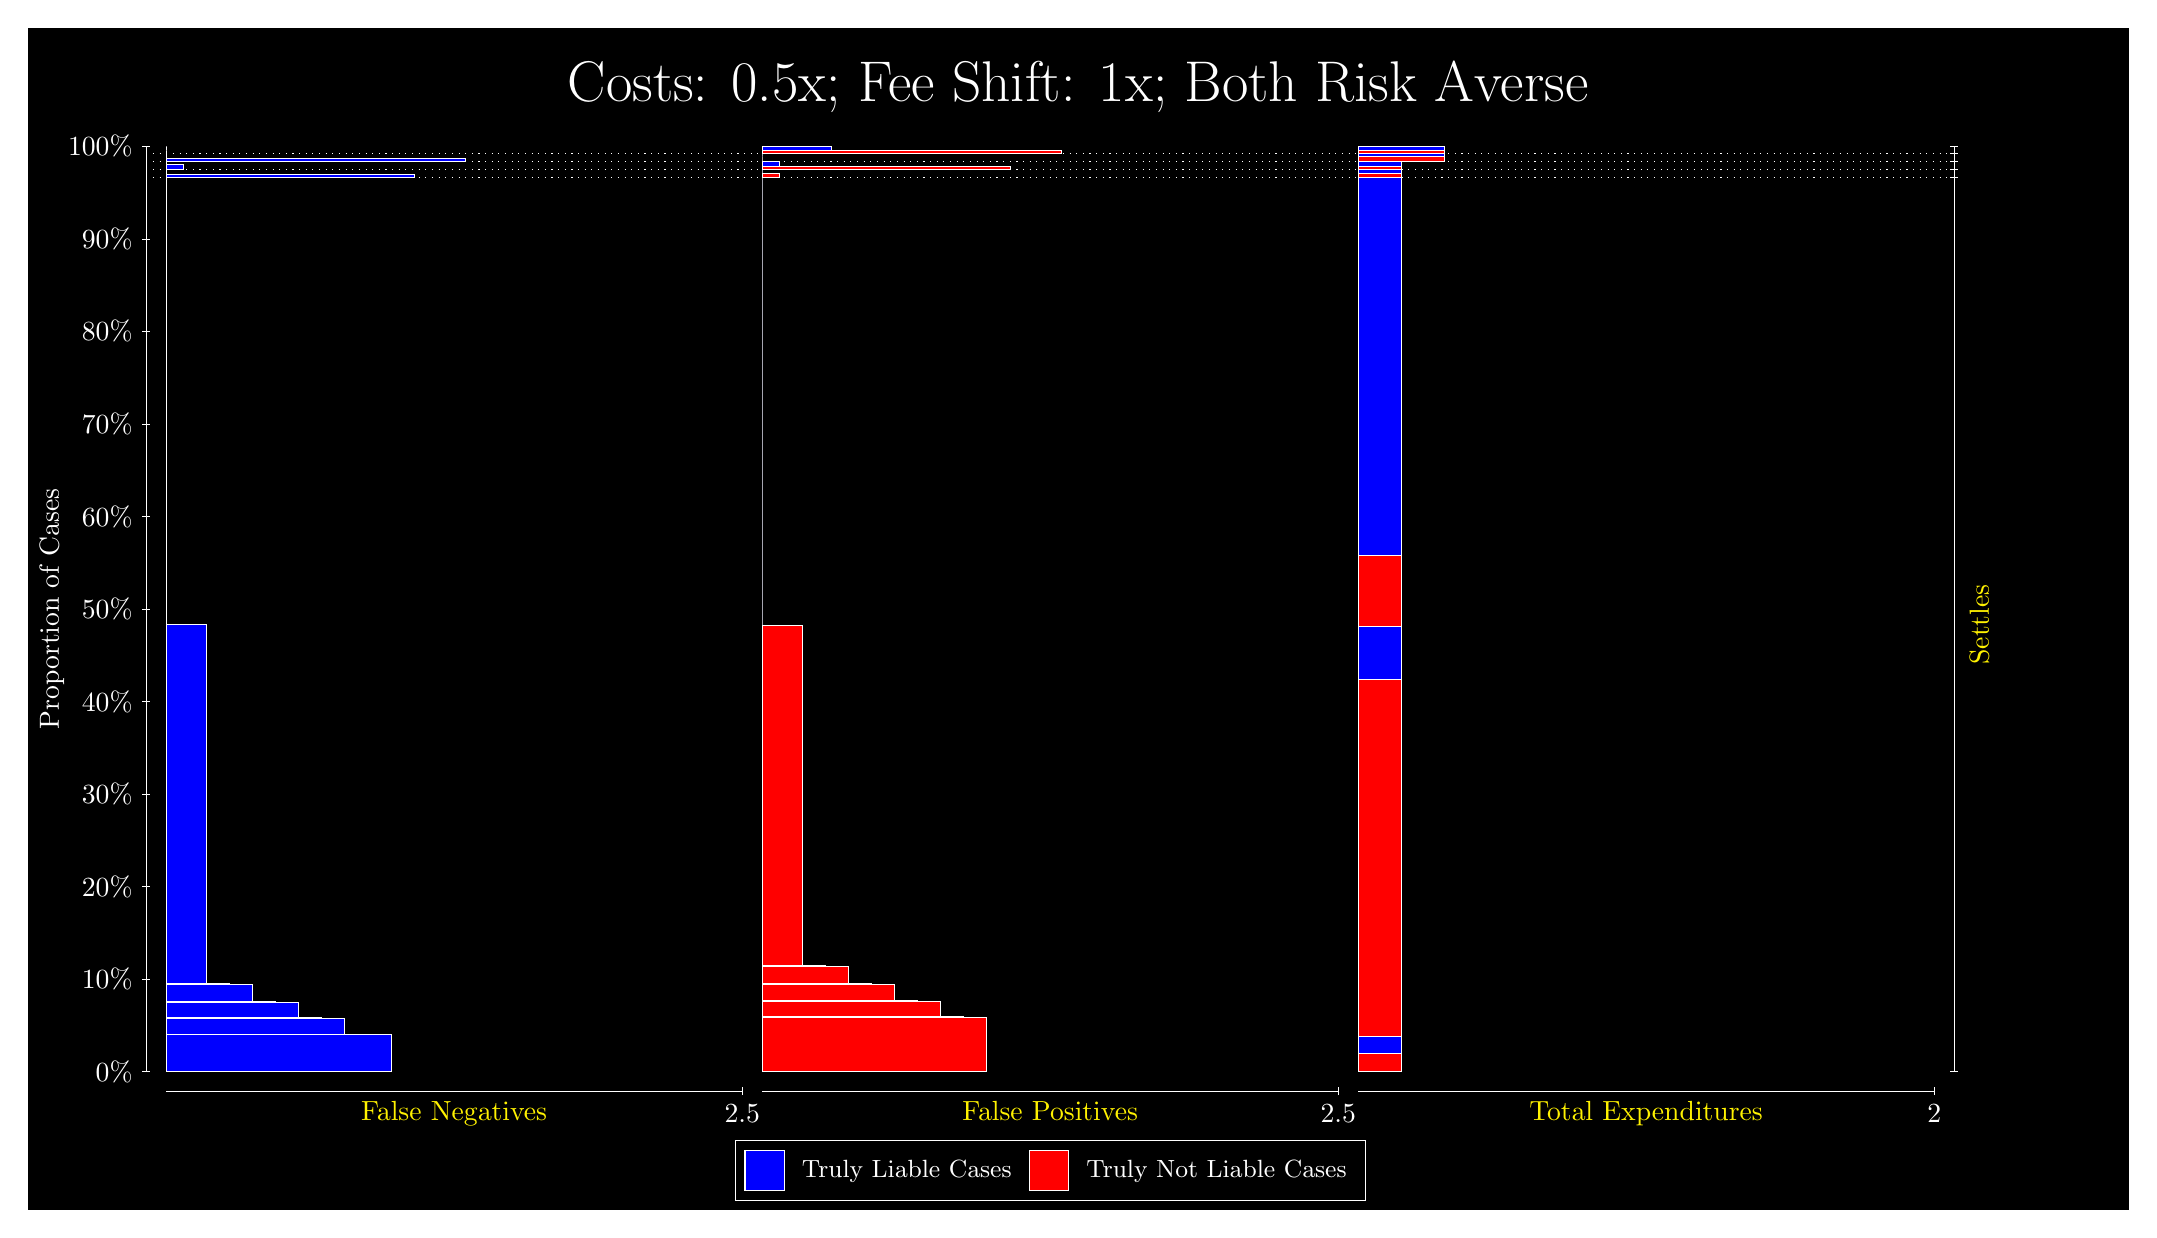
\begin{tikzpicture}
\draw[fill=black] (0,0) rectangle (26.667,15);
\draw[text=white] (0,13.5) rectangle (26.667,15) node[midway] {\huge Costs: 0.5x; Fee Shift: 1x; Both Risk Averse};
\draw[white, very thin] (1.5,1.75) -- (1.5,13.5);
\node[rotate=90, text=white, anchor=center] at (0.3, 7.625) {Proportion of Cases};
\draw[white, very thin] (1.45,1.75) -- (1.55,1.75);
\node[text=white, anchor=east] at (1.45, 1.75) {0\%};
\draw[white, very thin] (1.45,2.925) -- (1.55,2.925);
\node[text=white, anchor=east] at (1.45, 2.925) {10\%};
\draw[white, very thin] (1.45,4.1) -- (1.55,4.1);
\node[text=white, anchor=east] at (1.45, 4.1) {20\%};
\draw[white, very thin] (1.45,5.275) -- (1.55,5.275);
\node[text=white, anchor=east] at (1.45, 5.275) {30\%};
\draw[white, very thin] (1.45,6.45) -- (1.55,6.45);
\node[text=white, anchor=east] at (1.45, 6.45) {40\%};
\draw[white, very thin] (1.45,7.625) -- (1.55,7.625);
\node[text=white, anchor=east] at (1.45, 7.625) {50\%};
\draw[white, very thin] (1.45,8.8) -- (1.55,8.8);
\node[text=white, anchor=east] at (1.45, 8.8) {60\%};
\draw[white, very thin] (1.45,9.975) -- (1.55,9.975);
\node[text=white, anchor=east] at (1.45, 9.975) {70\%};
\draw[white, very thin] (1.45,11.15) -- (1.55,11.15);
\node[text=white, anchor=east] at (1.45, 11.15) {80\%};
\draw[white, very thin] (1.45,12.325) -- (1.55,12.325);
\node[text=white, anchor=east] at (1.45, 12.325) {90\%};
\draw[white, very thin] (1.45,13.5) -- (1.55,13.5);
\node[text=white, anchor=east] at (1.45, 13.5) {100\%};

\draw[white, very thin] (24.457,1.75) -- (24.457,13.5);
\draw[white, very thin] (24.407,1.75) -- (24.507,1.75);
\node[anchor=west] at (24.407, 1.75) {};
\draw[white, very thin] (24.407,13.105) -- (24.507,13.105);
\node[anchor=west] at (24.407, 13.105) {};
\draw[white, very thin] (24.407,13.208) -- (24.507,13.208);
\node[anchor=west] at (24.407, 13.208) {};
\draw[white, very thin] (24.407,13.309) -- (24.507,13.309);
\node[anchor=west] at (24.407, 13.309) {};
\draw[white, very thin] (24.407,13.41) -- (24.507,13.41);
\node[anchor=west] at (24.407, 13.41) {};
\draw[white, very thin] (24.407,13.5) -- (24.507,13.5);
\node[anchor=west] at (24.407, 13.5) {};

\draw[white, very thin, fill=blue] (1.75,1.75) rectangle (4.6044,2.2207);
\draw[white, very thin, fill=blue] (1.75,2.2207) rectangle (4.3116,2.2276);
\draw[white, very thin, fill=blue] (1.75,2.2276) rectangle (4.0188,2.4259);
\draw[white, very thin, fill=blue] (1.75,2.4259) rectangle (3.7261,2.4328);
\draw[white, very thin, fill=blue] (1.75,2.4328) rectangle (3.4333,2.6315);
\draw[white, very thin, fill=blue] (1.75,2.6315) rectangle (3.1406,2.646);
\draw[white, very thin, fill=blue] (1.75,2.646) rectangle (2.8478,2.8519);
\draw[white, very thin, fill=blue] (1.75,2.8519) rectangle (2.5551,2.8663);
\draw[white, very thin, fill=blue] (1.75,2.8663) rectangle (2.2623,7.431);
\draw[white, very thin, fill=red] (1.75,7.431) rectangle (1.75,13.105);
\draw[white, very thin, fill=blue] (1.75,13.105) rectangle (4.8971,13.149);
\draw[white, very thin, fill=red] (1.75,13.149) rectangle (1.75,13.208);
\draw[white, very thin, fill=blue] (1.75,13.208) rectangle (1.9696,13.266);
\draw[white, very thin, fill=red] (1.75,13.266) rectangle (1.75,13.309);
\draw[white, very thin, fill=blue] (1.75,13.309) rectangle (5.5558,13.351);
\draw[white, very thin, fill=red] (1.75,13.351) rectangle (1.75,13.41);
\draw[white, very thin, fill=red] (1.75,13.41) rectangle (1.75,13.45);
\draw[white, very thin, fill=blue] (1.75,13.45) rectangle (1.75,13.5);
\draw[white, very thin, fill=red] (9.3189,1.75) rectangle (12.173,2.4417);
\draw[white, very thin, fill=red] (9.3189,2.4417) rectangle (11.88,2.4485);
\draw[white, very thin, fill=red] (9.3189,2.4485) rectangle (11.588,2.6468);
\draw[white, very thin, fill=red] (9.3189,2.6468) rectangle (11.295,2.6537);
\draw[white, very thin, fill=red] (9.3189,2.6537) rectangle (11.002,2.86);
\draw[white, very thin, fill=red] (9.3189,2.86) rectangle (10.709,2.8745);
\draw[white, very thin, fill=red] (9.3189,2.8745) rectangle (10.417,3.0804);
\draw[white, very thin, fill=red] (9.3189,3.0804) rectangle (10.124,3.0948);
\draw[white, very thin, fill=red] (9.3189,3.0948) rectangle (9.8312,7.4235);
\draw[white, very thin, fill=blue] (9.3189,7.4235) rectangle (9.3189,13.105);
\draw[white, very thin, fill=red] (9.3189,13.105) rectangle (9.5384,13.164);
\draw[white, very thin, fill=blue] (9.3189,13.164) rectangle (9.3189,13.208);
\draw[white, very thin, fill=red] (9.3189,13.208) rectangle (12.466,13.251);
\draw[white, very thin, fill=blue] (9.3189,13.251) rectangle (9.5384,13.309);
\draw[white, very thin, fill=red] (9.3189,13.309) rectangle (9.3189,13.369);
\draw[white, very thin, fill=blue] (9.3189,13.369) rectangle (9.3189,13.41);
\draw[white, very thin, fill=red] (9.3189,13.41) rectangle (13.125,13.45);
\draw[white, very thin, fill=blue] (9.3189,13.45) rectangle (10.197,13.5);
\draw[white, very thin, fill=red] (16.888,1.75) rectangle (17.437,1.9848);
\draw[white, very thin, fill=blue] (16.888,1.9848) rectangle (17.437,2.1968);
\draw[white, very thin, fill=red] (16.888,2.1968) rectangle (17.437,6.7318);
\draw[white, very thin, fill=blue] (16.888,6.7318) rectangle (17.437,7.4013);
\draw[white, very thin, fill=red] (16.888,7.4013) rectangle (17.437,8.305);
\draw[white, very thin, fill=blue] (16.888,8.305) rectangle (17.437,13.105);
\draw[white, very thin, fill=red] (16.888,13.105) rectangle (17.437,13.164);
\draw[white, very thin, fill=blue] (16.888,13.164) rectangle (17.437,13.208);
\draw[white, very thin, fill=red] (16.888,13.208) rectangle (17.437,13.251);
\draw[white, very thin, fill=blue] (16.888,13.251) rectangle (17.437,13.309);
\draw[white, very thin, fill=red] (16.888,13.309) rectangle (17.986,13.369);
\draw[white, very thin, fill=blue] (16.888,13.369) rectangle (17.986,13.41);
\draw[white, very thin, fill=red] (16.888,13.41) rectangle (17.986,13.45);
\draw[white, very thin, fill=blue] (16.888,13.45) rectangle (17.986,13.5);
\draw[white, dotted] (1.5,13.105) -- (24.457,13.105);
\draw[white, dotted] (1.5,13.208) -- (24.457,13.208);
\draw[white, dotted] (1.5,13.309) -- (24.457,13.309);
\draw[white, dotted] (1.5,13.41) -- (24.457,13.41);
\draw[white, very thin] (1.75,1.5) -- (9.0689,1.5);
\node[text=yellow, anchor=north] at (5.4094, 1.5) {False Negatives};
\draw[white, very thin] (9.0689,1.45) -- (9.0689,1.55);
\node[text=white, anchor=north] at (9.0689, 1.45) {2.5};

\draw[white, very thin] (9.3189,1.5) -- (16.638,1.5);
\node[text=yellow, anchor=north] at (12.978, 1.5) {False Positives};
\draw[white, very thin] (16.638,1.45) -- (16.638,1.55);
\node[text=white, anchor=north] at (16.638, 1.45) {2.5};

\draw[white, very thin] (16.888,1.5) -- (24.207,1.5);
\node[text=yellow, anchor=north] at (20.547, 1.5) {Total Expenditures};
\draw[white, very thin] (24.207,1.45) -- (24.207,1.55);
\node[text=white, anchor=north] at (24.207, 1.45) {2};

\node[text=yellow, centered, rotate=90] at (24.777, 7.4273) {Settles};





\draw (12.978300999999998,1.5) node[draw=none] (baseCoordinate) {};
\begin{scope}[align=center]
        \matrix[scale=0.5, draw=white, below=0.5cm of baseCoordinate, nodes={draw}, column sep=0.1cm]{
            \node[rectangle, draw, minimum width=0.5cm, minimum height=0.5cm, fill=blue] {}; &
            \node[draw=none, font=\small, text=white] (B) {Truly Liable Cases}; &
            \node[rectangle, draw, minimum width=0.5cm, minimum height=0.5cm, fill=red] {}; &
            \node[draw=none, font=\small, text=white] (B) {Truly Not Liable Cases}; \\
            };
\end{scope}

\end{tikzpicture}
\end{document}